\documentclass[11pt,a4paper]{article}
\usepackage[UTF8,heading=true]{ctex}
\usepackage[a4paper,left=25mm,right=25mm,top=22mm,bottom=22mm]{geometry}
\usepackage{fontspec,xeCJK,graphicx,booktabs,array,amsmath,amssymb,float}
\usepackage[hidelinks]{hyperref}
\setmainfont{Times New Roman}
\setCJKmainfont{SimSun}[BoldFont=SimHei]
\setCJKsansfont{SimHei}
\setlength{\parindent}{2em}
\setlength{\parskip}{3pt}
\linespread{1.18}
\setlength{\tabcolsep}{5pt}
\setlength{\abovecaptionskip}{5pt}
\emergencystretch=1.5em
\widowpenalty=10000\clubpenalty=10000
\ctexset{section={format=\Large\bfseries},subsection={format=\large\bfseries},subsubsection={format=\normalsize\bfseries}}
\graphicspath{{figures/}}
\begin{document}

\section{问题四：波动电价下的购电与储能调度}

\subsection{建模思路与基本约定}

固定电价下，微网可以事先确定一天中的高低价时段，再安排电池转移电量。电价实时波动后，低价充电、高价放电的方向仍然成立，但具体价差不再提前可知。一次价格判断偏差，既可能使普通购电变贵，也可能改变电池在后续时段的余量。因此，本问需要预测未来价格，并据此重新优化购电和充放电安排，不能只用新价格重新计算原方案的费用。

本文保留问题二、三的供需预测与储能结构，分别建立零点订电和日内调整两条分支。前者只在每天零点确定当天普通订单；后者还可在6点、12点和18点结合新信息调整未执行部分。两者均不能提前使用未来真实电价、负载和光伏数据。负载与光伏仍分别预测，日内分支沿用问题三对官方光伏预报的融合与更新方法。

运行中采用光伏优先供负载的约定，剩余光伏在设备允许时充电；外网电既可直接供负载，也可给电池充电。充、放电效率各为90\%，不能利用的剩余电量不获得售电收益。跨日库存连续衔接，不继承问题一的每日首尾储电量相等约束。日内调整以零点订单为参照，每段只按执行前最后确定的订单结算一次。这些约定使两条分支可以在相同的物理和计费基础上比较。

以$d$表示自然日，$k=1,\ldots,144$表示十分钟区间，$\Delta t=1/6\,\mathrm{h}$。第$k$段为$[(k-1)\Delta t,k\Delta t)$，日内三个调整时点对应第37、73、109段开始前。原表循环排列的时间字段先映射到这一自然日顺序，输出时再逆向映射。为简化公式，将规划窗口内的连续区间记为$t\in\mathcal T_r$，$r$表示当前决策时点。$p_t$与$\widehat p_{t|r}$分别表示实际与预测电价，$\widehat L_{t|r}$、$\widehat V_{t|r}$为负载、光伏预测功率；$q_t$为普通订单电量，$S_t$为区间末电池内部储电量。其余决策量在相应公式处定义。

\subsection{电价规律与可用信息}

附件4共提供365天、52560个十分钟价格。为了解储能可利用的价差，先比较各时刻的平均价格及波动范围，如图\ref{fig:price}所示。

\begin{figure}[htbp]
\centering
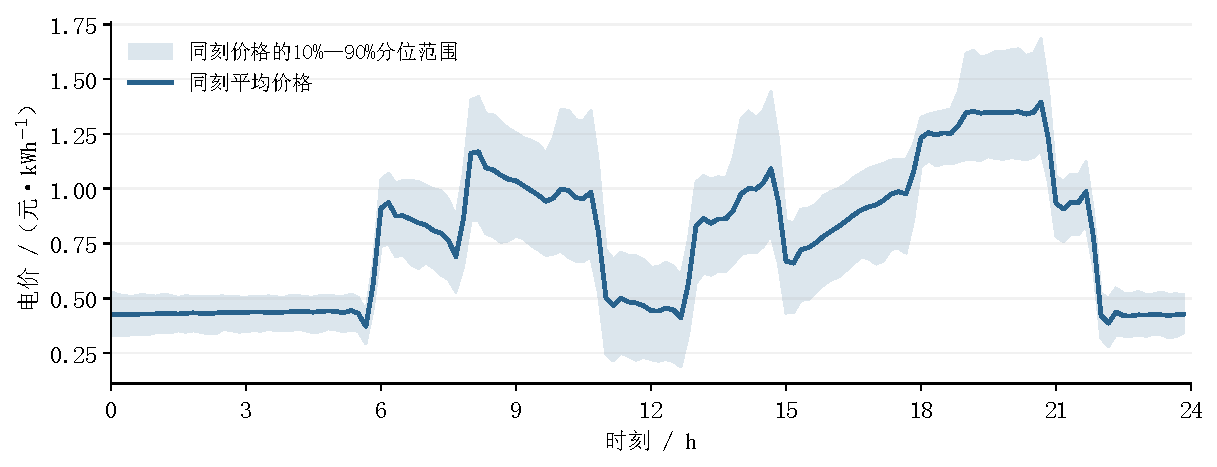
\includegraphics[width=.94\linewidth]{01_price_pattern.pdf}
\caption{全年同刻价格均值与10\%—90\%分位范围}
\label{fig:price}
\end{figure}

电价总体呈夜间较低、晚间较高的轮廓：05:40附近同刻均价约为0.3713元/kWh，20:40附近约为1.3952元/kWh；83.29\%的日最高价出现在19—22点。每日价格曲线与全年同刻均值曲线的平均相关系数约为0.9706，说明稳定的日内形状为价格判断提供了基础。与此同时，同刻价格仍存在明显波动，仅使用一条固定曲线会遗漏当天的整体偏移。

周周期也具有参考作用。上周同刻价格与当前价格的平均绝对差约为0.0466元/kWh，低于前一天同刻的0.0845元/kWh。因此，模型同时考虑相同星期几的历史价格和最近一周的价格变化。扣除同刻均值后，实际净负荷与价格偏差的相关系数约为0.9165，提示供需变化可能包含额外预测信息；实际建模使用当时可得的\textbf{预测}净负荷，不将这种关联解释为因果关系。

上述全年统计用于认识数据特征。逐日预测时，所有参考都严格截于决策时点。历史价格特征包括附件1给定曲线、过去四周相同星期几同刻的中位数、最近七天同刻中位数和上周同刻价格；辅助特征包括预测净负荷、目标星期、年内位置、预测提前量及当前发布时间。年内位置用正弦和余弦表示，以保持年末与年初的连续性。价格模型中的净负荷为$(\widehat L-\widehat V)/1000$，单位换成千千瓦以便数值处理，不在此处加入购电误差准备量。

日内分支进一步利用已经发生的价格。设$b_t$为同星期历史参考曲线，当日已完成区间集合为$\mathcal O_r$，构造
\begin{equation}
 a_r=\operatorname{median}_{t\in\mathcal O_r}(p_t-b_t),\qquad
 \ell_r=p_{r^-}-b_{r^-},
\end{equation}
其中$r^-$表示最后一个已完成区间。$a_r$反映今日整体偏差，$\ell_r$反映最近变化。对于距离当前$h$小时的当日目标区间，将$a_r$、$a_r\exp(-h/6)$和$\ell_r\exp(-h)$共同作为输入。两种尺度分别表达较缓的日内偏移和短时波动，是预设的特征形式；其实际作用还由拟合系数决定。零点尚无今日观测，或目标已跨到次日时，这三项均置零，避免把尚未发生的信息或今日异常直接带入次日。

\subsection{价格预测模型的建立与比较}

\subsubsection{历史参照、岭回归与提升树}

首先，以过去四周同星期同刻中位数作为透明基准；日内预测对当日部分加入已发生价格的中位偏差。该方法直接利用周周期，可以衡量更复杂方法是否带来了实际收益。

历史参考曲线之间高度相关，直接线性拟合可能用很大的正负系数相互抵消，以获得较小训练误差。这样的组合对参考曲线之间的小幅变化较敏感。为在利用多种参考的同时约束系数幅度，建立岭回归价格模型\cite{hoerl}。训练样本$i$的特征$x_{ij}$按当期训练集均值$\mu_j$和标准差$\sigma_j$标准化为$z_{ij}$，常量特征按单位尺度处理，求解
\begin{equation}
 \min_{\beta_0,\boldsymbol\beta}
 \sum_{i\in\mathcal I_r}\left(p_i-\beta_0-\sum_j\beta_jz_{ij}\right)^2
 +\lambda\sum_j\beta_j^2,\qquad \lambda=10.
 \label{eq:ridge}
\end{equation}
这里$\mathcal I_r$为当前可用历史样本集合。第一项要求预测接近实际价格，第二项限制过大的系数，截距$\beta_0$不受惩罚。标准化使惩罚不受特征单位支配。预测取
\begin{equation}
 \widehat p_{t|r}=\max\left\{0.001,\,\beta_0+\boldsymbol z_{t|r}^{\mathsf T}\boldsymbol\beta\right\},
\end{equation}
其中0.001仅为保证正价格的数值截断，不是题目规定的最低电价。

岭回归系数由历史数据估计，允许为负，也不要求和为一。解释时关注历史曲线、日内偏差与预测净负荷如何共同修正价格，而不把单个系数看成独立的因果作用。滚动拟合中，同星期参考和上周同刻价格的系数方向较稳定，净负荷系数则存在方向变化，说明其作用需要结合其他特征理解。式\eqref{eq:ridge}采用候选阶段固定的惩罚强度，本问不据此宣称其优于所有普通回归设定。

为检验非线性关系是否值得利用，再建立直方图梯度提升树\cite{friedman}。模型逐轮拟合前一轮的剩余误差，价格函数可表示为
\begin{equation}
 F_M(\boldsymbol x)=F_0(\boldsymbol x)+\gamma\sum_{m=1}^{M}h_m(\boldsymbol x),
 \qquad M=100,\quad\gamma=0.05.
\end{equation}
其中$h_m$为一棵回归树。分箱后的特征用于寻找划分位置，树能够表达历史价格与供需背景的交互，学习率则限制每轮修正幅度。初始每棵树最多15个叶节点，每叶至少50个训练样本，叶值采用强度为1的二次惩罚；后续检验叶节点数与历史窗口的敏感性。该方法比加法回归灵活，但整体解释需要依靠同条件比较，不能仅凭分裂次数判断现实因果。

两个学习模型每七天重拟合一次，使用最近56天的历史决策样本；不足时只使用已有历史。每个历史决策样本都按其当时信息重建，且仅在目标价格已经兑现后进入拟合。日内分支在四个决策时点更新输入和预测，不在每次预测时重新拟合参数。零点分支的日内价格特征始终为零，两条分支分别训练，避免引入额外信息权限。

\subsubsection{以调度费用而非单一预测误差选择模型}

价格误差的作用取决于当时的库存、功率限制和改单费用。例如，电池已经充满时，小幅改进低价预测未必改变购电；而高价缺电时，一次误判就可能增加五倍电价的紧急购电。因此，将三个候选分别接入相同分支的调度模型，统一初始库存，比较实际费用与紧急电量。表\ref{tab:candidates}给出首次比较结果；树模型在此处均为15叶版本。

\begin{table}[htbp]
\centering\small
\caption{同一起点下的价格候选比较（2025年2—12月）}
\label{tab:candidates}
\begin{tabular}{llrrr}
\toprule
分支 & 价格方法 & 价格MAE/(元/kWh) & 总费/万元 & 紧急电量/kWh \\
\midrule
零点订电 & 历史中位数 & 0.04984 & 1427.220 & 97728.89 \\
零点订电 & 岭回归 & 0.04472 & 1426.637 & 99205.19 \\
零点订电 & 提升树 & 0.03884 & 1425.518 & 98725.98 \\
日内调整 & 历史中位数 & 0.04676 & 1383.785 & 40144.52 \\
日内调整 & 岭回归 & 0.04442 & 1382.290 & 38733.80 \\
日内调整 & 提升树 & 0.03834 & 1382.063 & 40116.12 \\
\bottomrule
\end{tabular}
\end{table}

零点分支中，提升树相对岭回归减少费用11190.77元，且预测误差更小，故以提升树为深化基础。日内分支中，提升树仍然费用最低，但只比岭回归少2273.23元，约占后者总费的0.016\%，同时紧急电量增加1382.32 kWh；逐日比较为165天较便宜、169天较贵。本文因而在日内分支保留岭回归，以很小的费用让步换取较少紧急购电和更直接的解释。该选择是明确的费用与运行风险折中，并非岭回归在全部指标上占优。

\subsection{购电与储能模型的建立}

\subsubsection{供需准备与储能约束}

在决策时点$r$，将供需预测转换为区间电量，并沿用相应分支已有的误差准备量$m_{t|r}$：
\begin{equation}
 R_{t|r}=(\widehat L_{t|r}-\widehat V_{t|r})\Delta t+m_{t|r},\qquad
 n_t=\max(R_{t|r},0),\quad a_t=\max(-R_{t|r},0).
\end{equation}
$n_t$是准备后需要普通订单或储能补足的净需求，$a_t$为保守估计的剩余光伏。零点分支沿用过去28天、4小时分组的0.70加权分位准备；日内分支沿用过去28天、3小时分组的0.60加权分位准备，两者历史日期权重均按0.7逐日衰减。这里衰减的是历史误差的参考权重，不是把光伏预测乘以0.7。两条分支的准备策略保持各自既有版本，使价格候选比较只改变价格判断。

令$x_t$、$y_t$分别为外网与剩余光伏送往电池的外侧电量，$z_t$为电池向负载输出的外侧电量。储电变化满足
\begin{equation}
 S_t=S_{t-1}+\eta_c(x_t+y_t)-\frac{z_t}{\eta_d},\qquad
 \eta_c=\eta_d=0.9.
 \label{eq:storage}
\end{equation}
因此，100 kWh外侧电量充入后仅增加90 kWh库存，再放出最多提供81 kWh。储能套利必须覆盖这一损耗。容量和功率约束为
\begin{align}
 1200&\le S_t\le10800,\\
 x_t+y_t&\le K,\qquad K=5000\Delta t=\frac{2500}{3}\ \mathrm{kWh},\\
 0\le y_t&\le a_t,\qquad x_t\ge0,\qquad 0\le z_t\le K.
 \label{eq:limits}
\end{align}
每次求解以实际当前库存作为$S_{r^-}$。规划延伸到次日24点，因此零点窗口为48小时，6点、12点、18点依次为42、36、30小时。次日订单只辅助判断今日应保留多少电，不在当前提前签订。

为减弱窗口末端耗尽库存的倾向，在目标中设置$-\nu S_T$，其中$T$为窗口末段，$\nu=0.9p^{\rm base}_{0:00}$，使用附件1午夜电价作为固定参考。这是电池余量的规划价值，不是售电收入，不计入实际现金费用。

\subsubsection{零点一次订电模型}

零点分支将预计放电优先用于抵消净需求，要求$z_t\le n_t$。普通订单为
\begin{equation}
 q_t=n_t-z_t+x_t\ge0.
\end{equation}
结合式\eqref{eq:storage}—\eqref{eq:limits}，求解
\begin{equation}
 \min\ \sum_{t\in\mathcal T_0}\widehat p_{t|0}q_t-\nu S_T.
 \label{eq:dayahead}
\end{equation}
该模型通过误差准备预防缺电，不在计划内主动设置紧急购电变量。零点只保存当天144段普通订单，日内按真实供需执行；预测不足时，电池在放电功率和最低库存允许范围内补缺，仍不足的部分再紧急购入。这样既保留题目的一次订电权限，也区分了计划可行与实际供电保障。

\subsubsection{允许日内调整的购电模型}

日内分支需要把修改订单和未来可能的紧急购电放在同一目标下比较。令$e_t\ge0$为规划中的紧急购电量，$u_t\ge0$为预计不接收但仍需支付的普通订单电量，净需求平衡为
\begin{equation}
 q_t-x_t+z_t+e_t-u_t=n_t,\qquad z_t+e_t\le n_t,
 \label{eq:balance}
\end{equation}
并令$q_t\ge0$。其中，$q_t-x_t-u_t$表示普通电量扣除充电和未利用部分后对净需求的贡献。变量$u_t$允许模型在“保留多余订单”和“支付费用调减订单”之间权衡。

零点求解不设调整费，得到当天原计划$q_t^0$。此后仅对当天未执行区间集合$\mathcal D_r$调整，令$\delta_t\ge0$满足
\begin{equation}
 \delta_t\ge q_t-q_t^0,\qquad \delta_t\ge q_t^0-q_t,
 \qquad t\in\mathcal D_r.
\end{equation}
由于目标中调整系数为正，最优解取$\delta_t=|q_t-q_t^0|$，从而将绝对值费用转成线性形式。决策目标为
\begin{equation}
 \min\ \sum_{t\in\mathcal T_r}\widehat p_{t|r}(q_t+5e_t)
 +\frac12\sum_{t\in\mathcal D_r}\widehat p_{t|r}\delta_t-\nu S_T.
 \label{eq:intraday}
\end{equation}
约束包括式\eqref{eq:storage}—\eqref{eq:limits}及式\eqref{eq:balance}。窗口中的次日辅助订单没有当前日的零点合同，不计相对当前日原计划的调整费。已执行区间不再进入新的优化窗口，原计划$q^0$则始终保留。

设$q_t^F$为区间执行前最后确定的订单，$e_t^{\rm act}$为实际紧急购电。日内分支的真实费用为
\begin{equation}
 C_{4-3}=\sum_{d,k}\left[p_{d,k}q_{d,k}^{F}
 +\frac12p_{d,k}|q_{d,k}^{F}-q_{d,k}^{0}|
 +5p_{d,k}e_{d,k}^{\rm act}\right].
 \label{eq:cost}
\end{equation}
例如单价1元、原计划100 kWh，最终减为80 kWh时，相关费用为$80+0.5\times20=90$元；若最终增加到120 kWh，则为$120+0.5\times20=130$元。多次调整只据最终订单相对零点计划结算，不能重复累加中间调整记录。零点分支相应去掉式\eqref{eq:cost}的调整项，并取$q^F=q^0$。两式均以实际价格结算，规划时才使用预测价格。

\subsection{模型求解与实际运行}

价格确定后，两条分支的目标和约束均为线性形式，使用HiGHS求解。每个决策时点先读取已知供需、价格历史和实际库存，更新相应预测，再建立至次日24点的规划，保存当前允许执行或修改的当天订单。原计划与各次调整分别保留，便于按式\eqref{eq:cost}逐段核账。

真实执行以附件2给出的负载和光伏为准。先用光伏满足负载；若普通订单仍不足以覆盖剩余需求，则在功率和库存允许时放电，余缺紧急购入；若订单充足，则利用剩余光伏与订单余量充电，实际充电受功率及可用容量共同限制。未利用订单仍收费，未利用光伏不增加收益。该执行规则按供需情况区分充电与放电分支，保证实际运行不同时充放电。计划模型未加入整数互斥变量，已保存求解结果中也未出现同时充放电，但不把这一观测替代所有输入下的互斥证明。

2025年1月1日从题给6000 kWh及既定首日订单启动，1月用于初始化和历史积累。候选比较统一从2月1日8592.69356093 kWh开始，正式统计至12月31日，共334天；之后每日库存连续传递。初次试算中各方案自行初始化会造成2月1日库存不同，故最终采用统一起点结果，避免把初始电量优势计作模型优势。

\subsection{深化后的结果与运行表现}

零点分支在特征不变时比较了7、15、31叶树，并检验28、56、84天历史窗口。31叶版本相对原15叶减少6605.53元，总费为14248570.87元，价格MAE由0.03884降至0.03818元/kWh，故采用该版本。日内分支尝试以历史中位曲线为底、只拟合价格偏差的残差式岭回归，但费用和紧急电量均未改善，因而保留完整岭回归。两条当前方案的费用构成见表\ref{tab:final}。

\begin{table}[htbp]
\centering\small
\caption{两条分支的334天实际费用与库存}
\label{tab:final}
\begin{tabular}{lrr}
\toprule
指标 & 零点订电：31叶提升树 & 日内调整：完整岭回归 \\
\midrule
普通购电费/元 & 13613522.32 & 13327163.05 \\
调整费/元 & 0.00 & 268515.82 \\
紧急购电费/元 & 635048.55 & 227222.48 \\
总费用/元 & 14248570.87 & 13822901.35 \\
紧急购电量/kWh & 98756.33 & 38733.80 \\
期末储电量/kWh & 8692.34 & 7918.81 \\
\bottomrule
\end{tabular}
\end{table}

日内方案虽增加调整费，但普通费用和紧急费用更低，合计比零点方案少425669.52元，约2.99\%。该差额包括供需信息、准备策略、价格方法和调整权限的共同作用，不宜全部归因于日内电价更新。表\ref{tab:days}列出四个指定日期的结果摘要，其中普通订单是付费计划量，不等同于最终全部接收利用的电量。

\begin{table}[htbp]
\centering\footnotesize
\caption{指定日期的购电与储电结果摘要}
\label{tab:days}
\begin{tabular}{llrrrr}
\toprule
分支 & 日期 & 普通订单/kWh & 紧急购电/kWh & 日末储电/kWh & 总费/元 \\
\midrule
零点订电 & 03-20 & 62329.63 & 329.13 & 1376.30 & 41909.16 \\
零点订电 & 06-21 & 42375.21 & 0.00 & 10380.22 & 20358.11 \\
零点订电 & 09-23 & 68066.93 & 10.23 & 2592.35 & 44700.97 \\
零点订电 & 12-21 & 94612.77 & 0.00 & 9798.14 & 71357.71 \\
日内调整 & 03-20 & 61795.52 & 93.27 & 1311.14 & 40921.66 \\
日内调整 & 06-21 & 42176.92 & 14.64 & 10800.00 & 20204.97 \\
日内调整 & 09-23 & 67751.81 & 11.32 & 3463.77 & 45250.33 \\
日内调整 & 12-21 & 93283.52 & 20.53 & 8131.62 & 71876.82 \\
\bottomrule
\end{tabular}
\end{table}

为了判断费用优势是否在不同月份保持一致，图\ref{fig:months}保留了逐月比较中的正负差额。零点31叶树相对15叶树在7个月节费、4个月增费，逐日为179天节费、149天增费、6天相同；日内岭回归相对原提升树也有正负交替。这说明年度总费优势不能解释为每个月或每天都更好。对于日内方案，较少紧急电量与结构可解释性仍是选择依据，月度图不改变其存在小额经济让步的事实。

\begin{figure}[htbp]
\centering
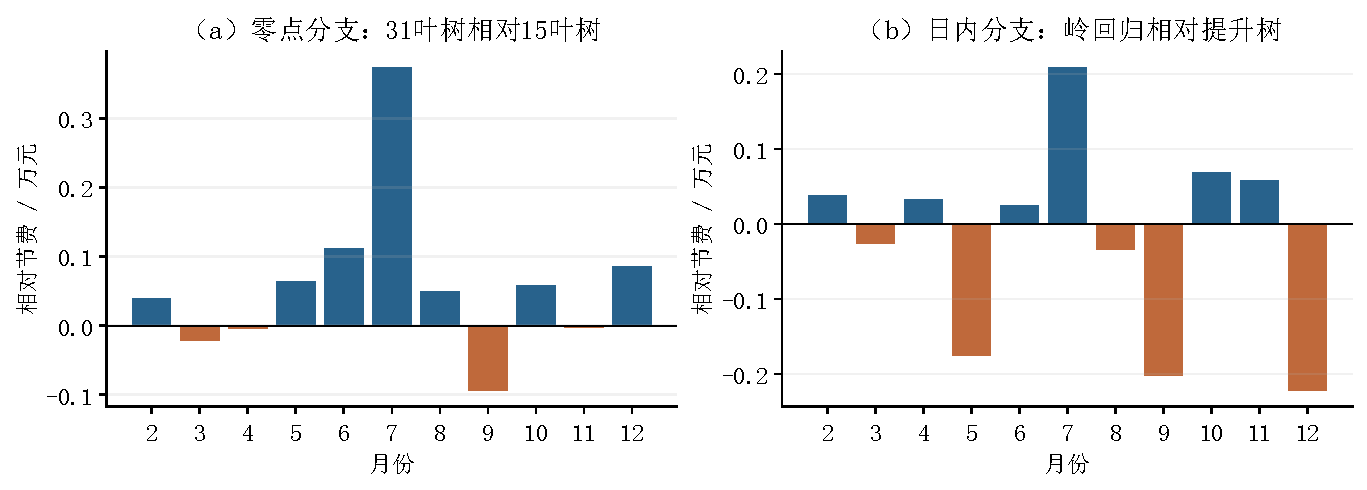
\includegraphics[width=\linewidth]{02_monthly_comparison.pdf}
\caption{两条分支各自对照下的月度节费，正值表示图题中前者更省}
\label{fig:months}
\end{figure}

\subsection{敏感性检验、信息价值与风险分析}

\subsubsection{结构与参数改变是否支持当前选择}

零点分支删除预测净负荷后，相对原15叶完整树增费5392.23元，说明这一供需参考在该结构下有帮助。但只保留历史价格的简化模型仅增费7.59元，同时高价MAE由0.05124升至0.06828元/kWh，表明特征能够相互补偿，预测改进也未必按比例转化为节费。在所测窗口、叶节点和特征变体中，树模型总费均低于初始岭回归，支持零点分支采用这一模型家族。

图\ref{fig:validation}(a)展示每棵树叶节点数的影响。31叶在本年结果中最低，但该改进并未改善全部风险指标：紧急费下降3783.04元，紧急电量却增加30.35 kWh。这说明改进主要与缺电发生时段及其价格有关，不能写成完全消除了紧急风险。

日内分支的残差式岭回归在惩罚强度10时，相对完整模型增费759.32元，紧急电增加150.84 kWh；强度1和100时同样增费，故不保留这一结构。残差式再删除净负荷后，相对同样的残差式模型增费2368.29元。这里采用同结构对照，不把相对完整模型的全部费用差归于某一个特征。

\subsubsection{日内价格更新是否值得保留}

为单独评价价格信息，保留原供需更新、实际库存反馈和调整权限，仅改变今日已发生价格是否进入后续预测。全天保持零点价格判断，相对完整更新增费274.45元。分别不使用6点、12点和18点的价格更新，费用变化为$+59.37$、$-27.40$和$+312.58$元，如图\ref{fig:validation}(b)所示。

\begin{figure}[htbp]
\centering
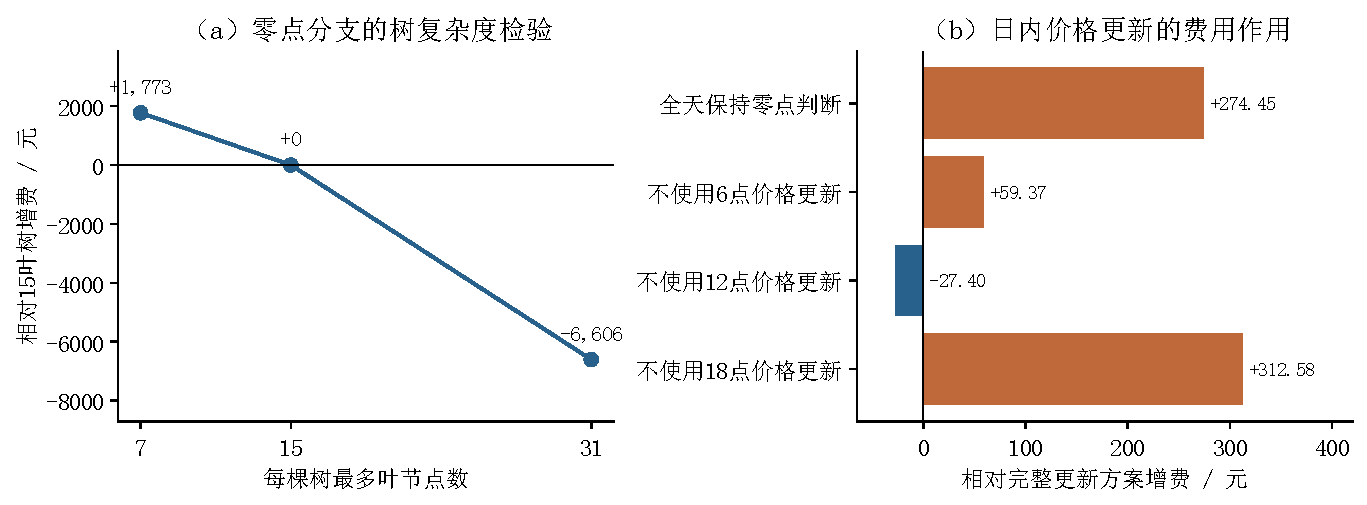
\includegraphics[width=\linewidth]{03_validation.pdf}
\caption{树复杂度与日内价格更新的同条件检验}
\label{fig:validation}
\end{figure}

日内价格更新的额外收益较小，18点的修正相对更有价值。12点不更新反而略省，说明信息增加不保证本次控制决策更省钱；该差额很小，尚不足以据此取消统一的四次更新结构。各次对照会改变后续同一条库存轨迹，作用重叠，费用差不能相加。这一检验也没有取消日内供需信息，不能用于否定光伏预报和调整权限的价值。

\subsubsection{高价风险、期末库存与检验边界}

将真实价格最高的5\%区间单列，阈值为1.3246元/kWh，共2407段。零点31叶方案在这些区间紧急购电46086.96 kWh，低于原15叶方案的46430.63 kWh；日内岭回归为14665.07 kWh，仍存在高价补电风险。进一步回看连续高价区间，数据中最长连续高价达到3小时，有限库存和充放电功率使电池无法无限缓冲供需偏差。因此，本问的改善是降低给定历史条件下的费用，不能理解为对所有连续高价过程提供充分保障。

不同方案期末库存不一，还需排除少留电造成的费用优势。以低、中、高三档参考价$\rho$估计剩余可放电量的价值，定义比较指标
\begin{equation}
 J(\rho)=C-\rho\eta_d\max(S_{\rm end}-1200,0),\qquad
 \rho\in\{0.336675,\ 0.7267,\ 1.3246\}.
\end{equation}
该指标仅用于比较，不改变实际账单。零点31叶相对15叶在三档下仍节费5890.24—6423.72元，支持其改善不只是消耗库存。日内原提升树经同样估值后仍比岭回归便宜，进一步表明选择岭回归是一项有经济代价的折中。

此外，在供需预测和控制结构保持不变时，以提前获知真实价格构造不可执行参照。零点和日内分支的费用差分别为65545.16元和94749.67元，占当前费用的0.460\%和0.685\%。这一结果提示当前结构中继续精细改进价格预测的收益可能有限，但参照并非全问题的理论最优下界，不能据此排除价格与供需联合优化的潜在价值。

对已保存结果的另一条核算路径重新检查了供需平衡、库存递推、功率限制、信息截止时点和逐段费用。深化批次865728个实际区间的总账最大差约为$1.86\times10^{-9}$元，支持结果的数值一致性。模型训练逐次遵守时间先后，但方案和参数比较使用了同一年的整体表现，因此现有证据属于2025年的滚动检验及有限敏感性分析，尚不能代表独立年份的泛化表现。

\subsection{本问结论}

波动价格下，本文以合法历史信息预测未来价格，再通过线性规划安排普通购电与储能。零点订电采用31叶直方图提升树，日内调整采用完整岭回归，2025年2—12月总费分别为14248570.87元和13822901.35元。前者在所测候选中取得较好的费用表现，后者在接近最低费用的同时减少紧急购电并保留清晰的解释。实际费用比较、参数检验、日内信息对照和期末库存估值共同支持这一选择，同时保留单日增费、高价补电以及跨年表现未验证的适用边界。

\begin{thebibliography}{9}
\bibitem{hoerl} Hoerl A E, Kennard R W. Ridge regression: Biased estimation for nonorthogonal problems[J]. Technometrics, 1970, 12(1): 55--67.
\bibitem{friedman} Friedman J H. Greedy function approximation: A gradient boosting machine[J]. The Annals of Statistics, 2001, 29(5): 1189--1232.
\end{thebibliography}
\end{document}

